\section{Position}
\begin{enumerate}
\item IDA打开查看函数列表确认没有加壳,直接静态分析。\\
\item 
	\begin{enumerate}
	\item Shift + F12 打开Strings窗口,查找字符串“\lstinline$Correct!\n$”和“\lstinline$Wrong\n$”\\
	\item 如果无字符串“\lstinline$Correct!\n$”,右键 任一字符串,选择菜单项“Setup”、、
	\item 勾选“Unicode”前复选框,点击OK。字符串“\lstinline$Correct!\n$”出现\\
		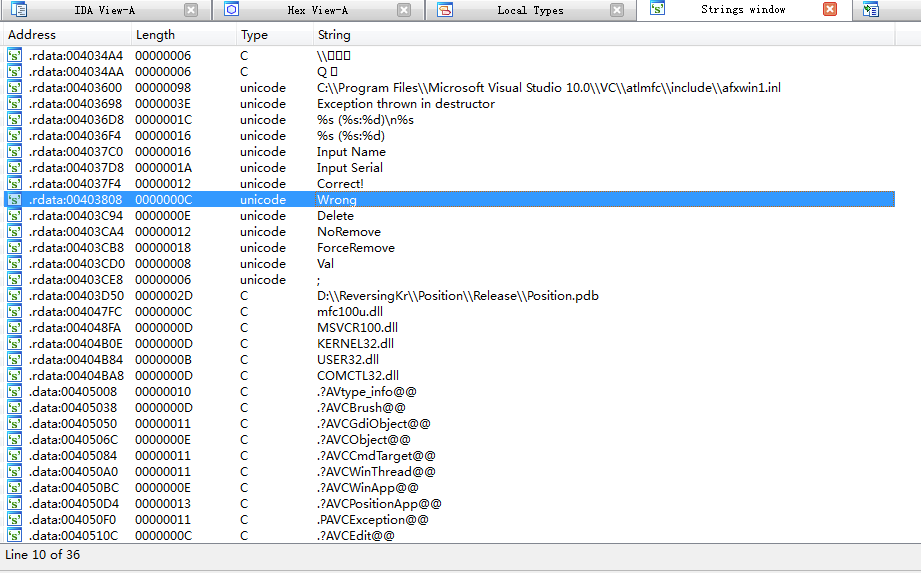
\includegraphics[width=10cm]{position-str} \\
	\item 双击 转到字符串定义,\\
	\item 双击 交叉引用(DATA XREF)的函数名,跳转到对应函数定义,\\
	\item 空格 切换为Graph View分析函数功能 \\
	\end{enumerate} 
\item 
	 函数\lstinline$sub_401740$返回值非零,分析显示字符串“\lstinline$Correct!\n$”分支,\\
	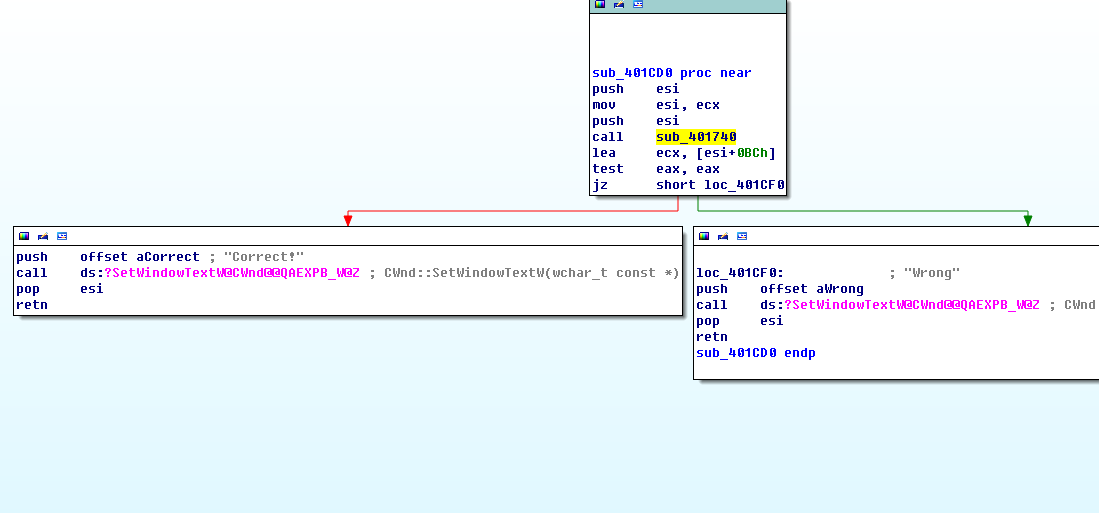
\includegraphics[width=10cm]{position-judge} \\
	双击 函数\lstinline$sub_401740$跳转到定义,分析算法: \\
	获取name存放在CString\lstinline$[esp+var_18]$中:\\
	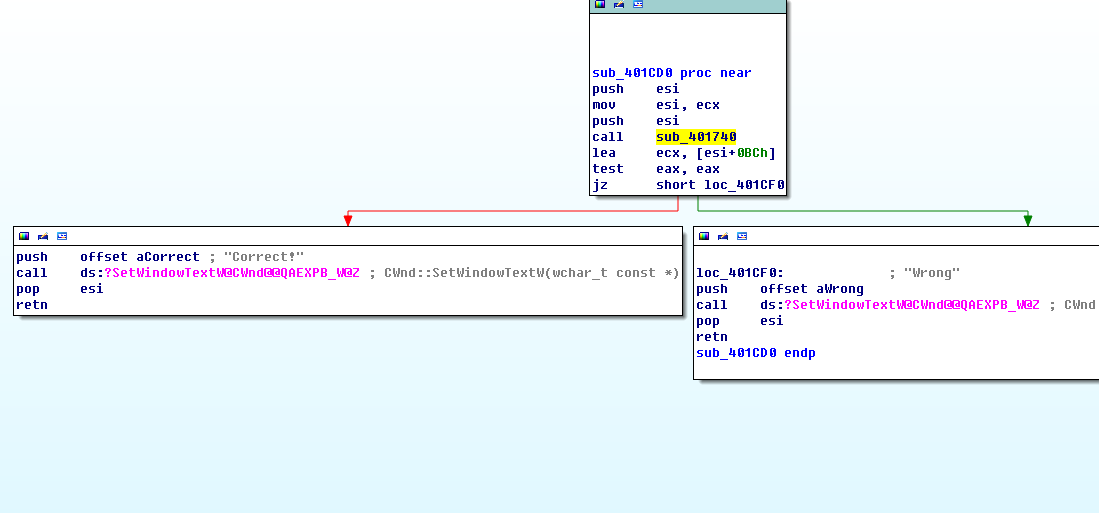
\includegraphics[width=10cm]{position-judge} \\
	校验长度是否为4:\\
	\begin{lstlisting}
	mov     ecx, [ebp+var_18]
	cmp     dword ptr [ecx-0Ch], 4
	\end{lstlisting}
	校验字符是否在范围:a-z \\
	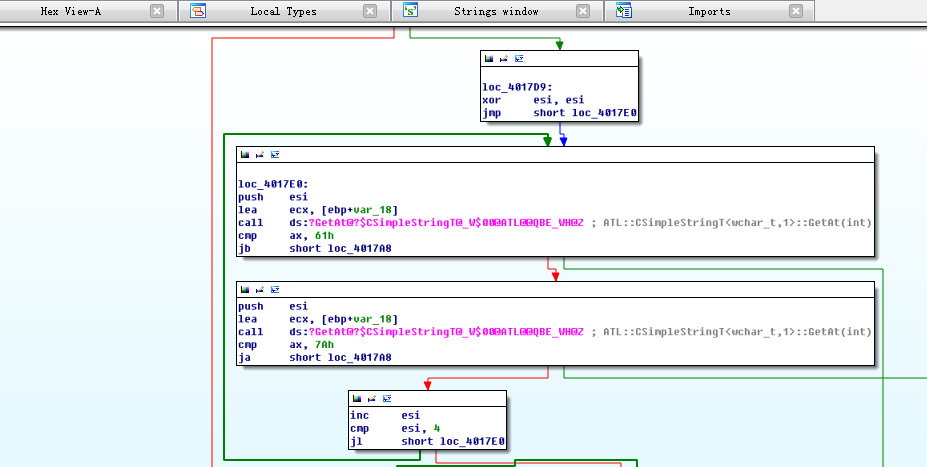
\includegraphics[width=10cm]{position-check-char} \\
	校验字符是否重复:\\
	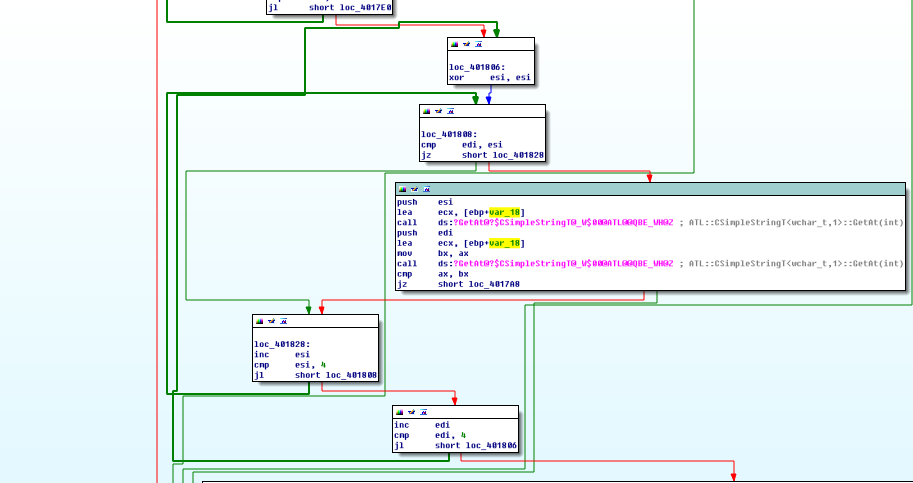
\includegraphics[width=10cm]{position-check-repeat} \\
	获取serial存放在CString\lstinline$[esp+var_14]$中,判断第5个字符是否‘-’:\\
	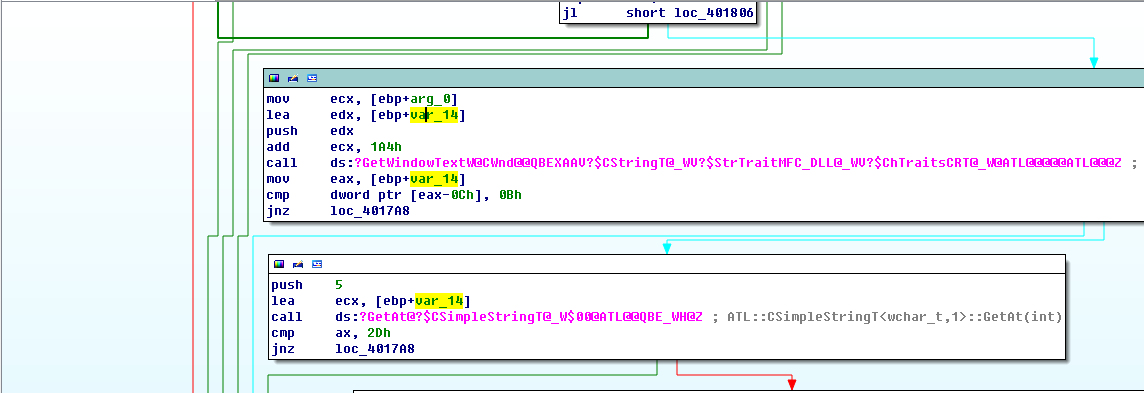
\includegraphics[width=10cm]{position-serial} \\
	关键算法分析:(\lstinline$var_26$并未真实存储,而是直接用于计算了)\\
Name[0]		二进制取1、2、3、4、5位 add 5 存放	\lstinline$var_20	var_1F	var_1E	var_1D	var_1C$\\
Name[1]		二进制取1、2、3、4、5位 add 1 存放	\lstinline$var_28	var_27	var_26	var_25	var_24$\\

\lstinline$var_20 + var_26$	转换字符存储	\lstinline$[esp+var_10] CString	[0] == Serial[0]$\\
\lstinline$var_1D + var_25$	转换字符存储	\lstinline$[esp+var_10] CString	[0] == Serial[1]$\\
\lstinline$var_1F + var_24$	转换字符存储	\lstinline$[esp+var_10] CString	[0] == Serial[2]$\\
\lstinline$var_1E + var_28$	转换字符存储	\lstinline$[esp+var_10] CString	[0] == Serial[3]$\\
\lstinline$var_1C + var_27$	转换字符存储	\lstinline$[esp+var_10] CString	[0] == Serial[4]$\\



Name[2]		二进制取1、2、3、4、5位 add 5 存放	\lstinline$var_20	var_1F	var_1E	var_1D	var_1C$\\
Name[3]		二进制取1、2、3、4、5位 add 1 存放	\lstinline$var_28	var_27	var_26	var_25	var_24$\\

\lstinline$var_20 + var_26$	转换字符存储	\lstinline$[esp+var_10] CString	[0] == Serial[6]$\\
\lstinline$var_1D + var_25$	转换字符存储	\lstinline$[esp+var_10] CString	[0] == Serial[7]$\\
\lstinline$var_1F + var_24$	转换字符存储	\lstinline$[esp+var_10] CString	[0] == Serial[8]$\\
\lstinline$var_1E + var_28$	转换字符存储	\lstinline$[esp+var_10] CString	[0] == Serial[9]$\\
\lstinline$var_1C + var_27$	转换字符存储	\lstinline$[esp+var_10] CString	[0] == Serial[10]$\\
	前两个字符与后两个字符处理一样:\\
	\begin{lstlisting}[language=C]
#include "stdio.h"
#define LEN 5
int main()
{
	char VAR_20[LEN] = { 0 };
	char VAR_28[LEN] = { 0 };
	int ch_a = 0x61;
	int ch_z = 0x7a;
	int i = ch_a;
	for (; i < ch_z+1; i++)
	{
		int j = ch_a;
		for (; j < ch_z + 1; j++)
		{
			if (i == j)
				continue;
			else {
				int k;
				int l, m;
				for (k = 0; k < LEN; k++)
				{
					l = i >> k;
					m = j >> k;
					l = 1 & l;
					m = 1 & m;
					VAR_20[k] = l + 5;
					VAR_28[k] = m + 1;
				}
				printf("%c%c\t", i, j);
printf("%d", VAR_20[0x20-0x20] + VAR_28[0x28-0x26]);	// var_20 + var_26
printf("%d", VAR_20[0x20-0x1D] + VAR_28[0x28-0x25]);	// var_1D + var_25
printf("%d", VAR_20[0x20-0x1F] + VAR_28[0x28-0x24]);	// var_1F + var_24
printf("%d", VAR_20[0x20-0x1E] + VAR_28[0x28-0x28]);	// var_1D + var_28
printf("%d", VAR_20[0x20-0x1C] + VAR_28[0x28-0x27]);	// var_1D + var_27
				printf("\n");
			}
		}
	}
	printf("\n");
	getchar();
}
	\end{lstlisting}
	利用重定向,将标准输出到文件1.txt, 分别搜索76876与77776\\
	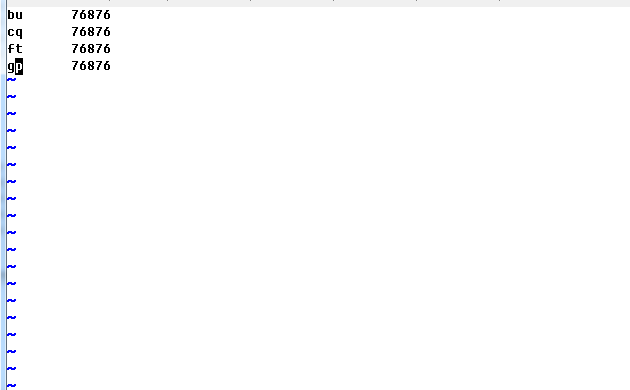
\includegraphics[width=10cm]{position-76876} \\
	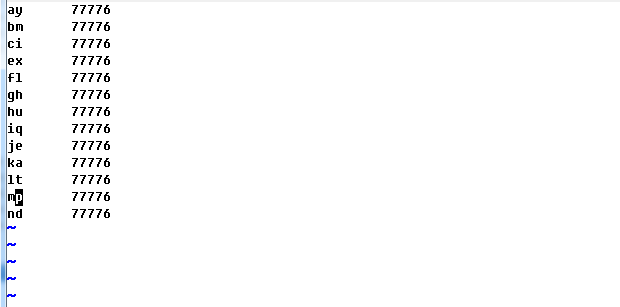
\includegraphics[width=10cm]{position-77776} \\
	有三组name满足条件(serial=76876-77776,name=***p):bump、cqmp、ftmp \\
	flag : ``bump''
\end{enumerate}